\documentclass[12pt,a4paper]{article}
\usepackage{amsmath}
\usepackage{amsfonts}
\usepackage{amssymb}
\usepackage{graphicx}
\usepackage{secdot}
\usepackage[left=2cm,right=2cm,top=2cm,bottom=2cm]{geometry}

\author{Shibayan Biswas, AE21B109,\\ Department of Aerospace Engineering,\\ IIT Madras}

\title{Assignment - 2}

\date{September 07, 2022}

\begin{document}

\maketitle
\hline
\section{Methods for Finding Solution Matrix in Octave:}
There are various methods for finding the Solution Matrix for a system of linear equations. As per the given assignment we have to perform 3 methods that are mentioned. So in this section, I have provided a brief overview of the 3 methods and the tasks performed related to them; shown below:
\subsection{Method- 1 (Gaussian Elimination Method):}
In mathematics, Gaussian elimination, also known as row reduction, is an algorithm for solving systems of linear equations. It consists of a sequence of operations performed on the corresponding matrix of coefficients. This method can also be used to compute the rank of a matrix, the determinant of a square matrix, and the inverse of an invertible matrix. The method is named after Carl Friedrich Gauss (1777–1855) although some special cases of the method—albeit presented without proof—were known to Chinese mathematicians as early as circa 179 AD.\\
\\To perform row reduction on a matrix, one uses a sequence of elementary row operations to modify the matrix until the lower left-hand corner of the matrix is filled with zeros, as much as possible. There are three types of elementary row operations:
\begin{itemize}
\item Swapping two rows
\item Multiplying a row by a non-zero number
\item Adding a multiple of one row to another row (subtraction can be achieved by multiplying one row with -1 and adding the result to another row)
\end{itemize}
\\Using these operations, a matrix can always be transformed into an upper triangular matrix, and in fact one that is in row echelon form. Once all of the leading coefficients (the leftmost non-zero entry in each row) are 1, and every column containing a leading coefficient has zeros elsewhere, the matrix is said to be in reduced row echelon form. This final form is unique; in other words, it is independent of the sequence of row operations used. Using row operations to convert a matrix into reduced row echelon form is sometimes called Gauss–Jordan elimination. In this case, the term Gaussian elimination refers to the process until it has reached its upper triangular, or (un reduced) row echelon form. For computational reasons, when solving systems of linear equations, it is sometimes preferable to stop row operations before the matrix is completely reduced.
\subsection{Method- 2 (Using inverse (inv()) Method):}
For a given matrix containing the the coefficients of the variables (for each equation for a system of equations) and for a given vector containing the values of constants (for each equation for a system of equations), the solution matrix (for the system of linear equations) in Octave can be found by multiplying the inverse of the matrix- that can be found out using the inverse (inv()) Method; and the vector.
\subsection{Method- 3 (Using backslash ($\backslash$) operator):}
For a given matrix containing the the coefficients of the variables (for each equation for a system of equations) and for a given vector containing the values of constants (for each equation for a system of equations), the solution matrix (for the system of linear equations) in Octave can be found by using the backslash ($\backslash$) operator between the matrix and the vector.
\subsection{Plot of L$\infty$ v/s Matrix Size (n):}
L$\infty$ norm gives the largest magnitude among each element of a vector. In L$\infty$ norm, only the largest element has any effect. So, for example, if your vector represents the cost of constructing a building, by minimizing L$\infty$ norm we are reducing the cost of constructing the building. The plot of the L$\infty$  norm of error between the Method 1 and Method 2 and Method 1 and Method 3 against matrix size ’n’ up to 1000 is shown below in the figure:
\begin{figure}[!ht]
	\begin{center}
		\framebox{
			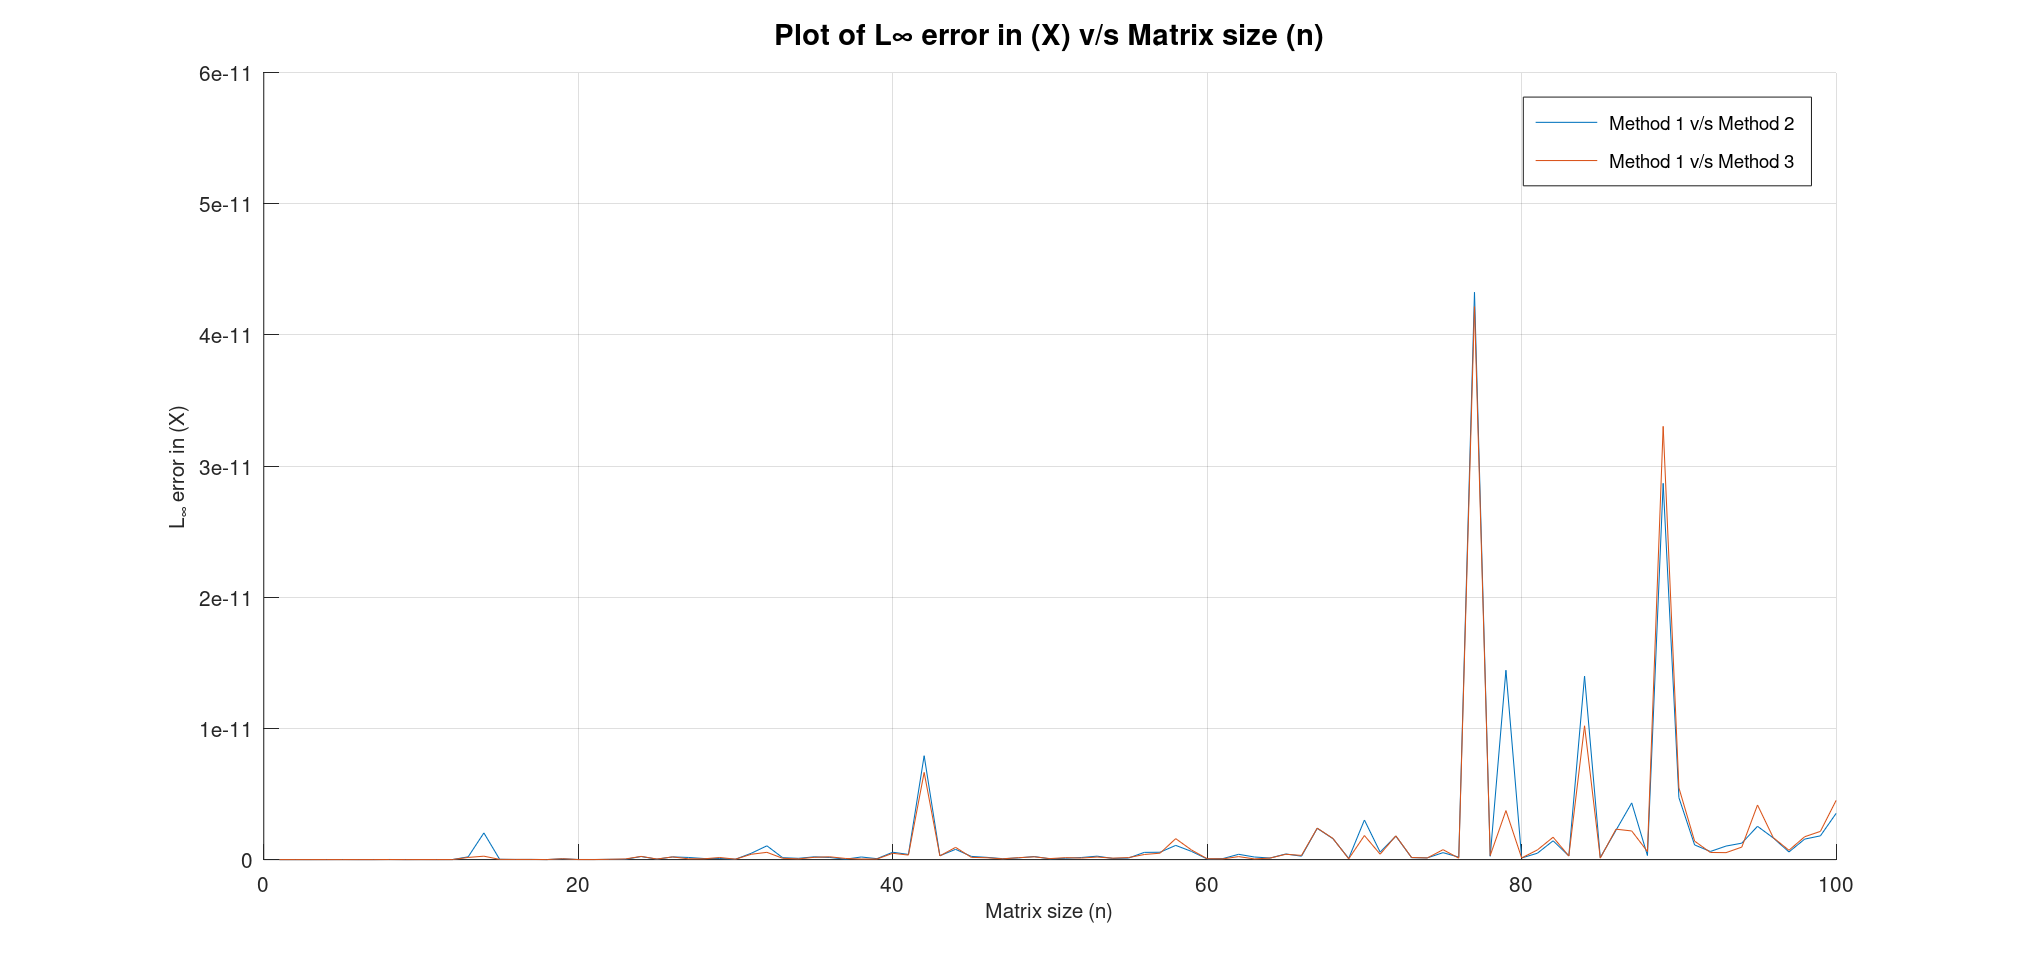
\includegraphics[scale=0.2]{Figure_1.png}
		}
	\end{center}
	\caption{Plot of L$\infty$ v/s Matrix Size (n)}
\end{figure}
\subsection{Plot of Wall Clock Time (t) v/s Matrix size (n):}
In this section I have shown the plot for the wall clock time for each method discussed in the previous sections. Wall time, also called real-world time or wall-clock time, refers to elapsed time as determined by a chronometer such as a wristwatch or wall clock. (The reference to a wall clock is how the term originally got its name.) Wall time differs from time as measured by counting microprocessor clock pulses or cycles. In this particular assignment, Method 3 has the least wall clock time, followed by Method 2 and then Method 1. The required plot is shown below in the figure:
\begin{figure}[!ht]
	\begin{center}
		\framebox{
			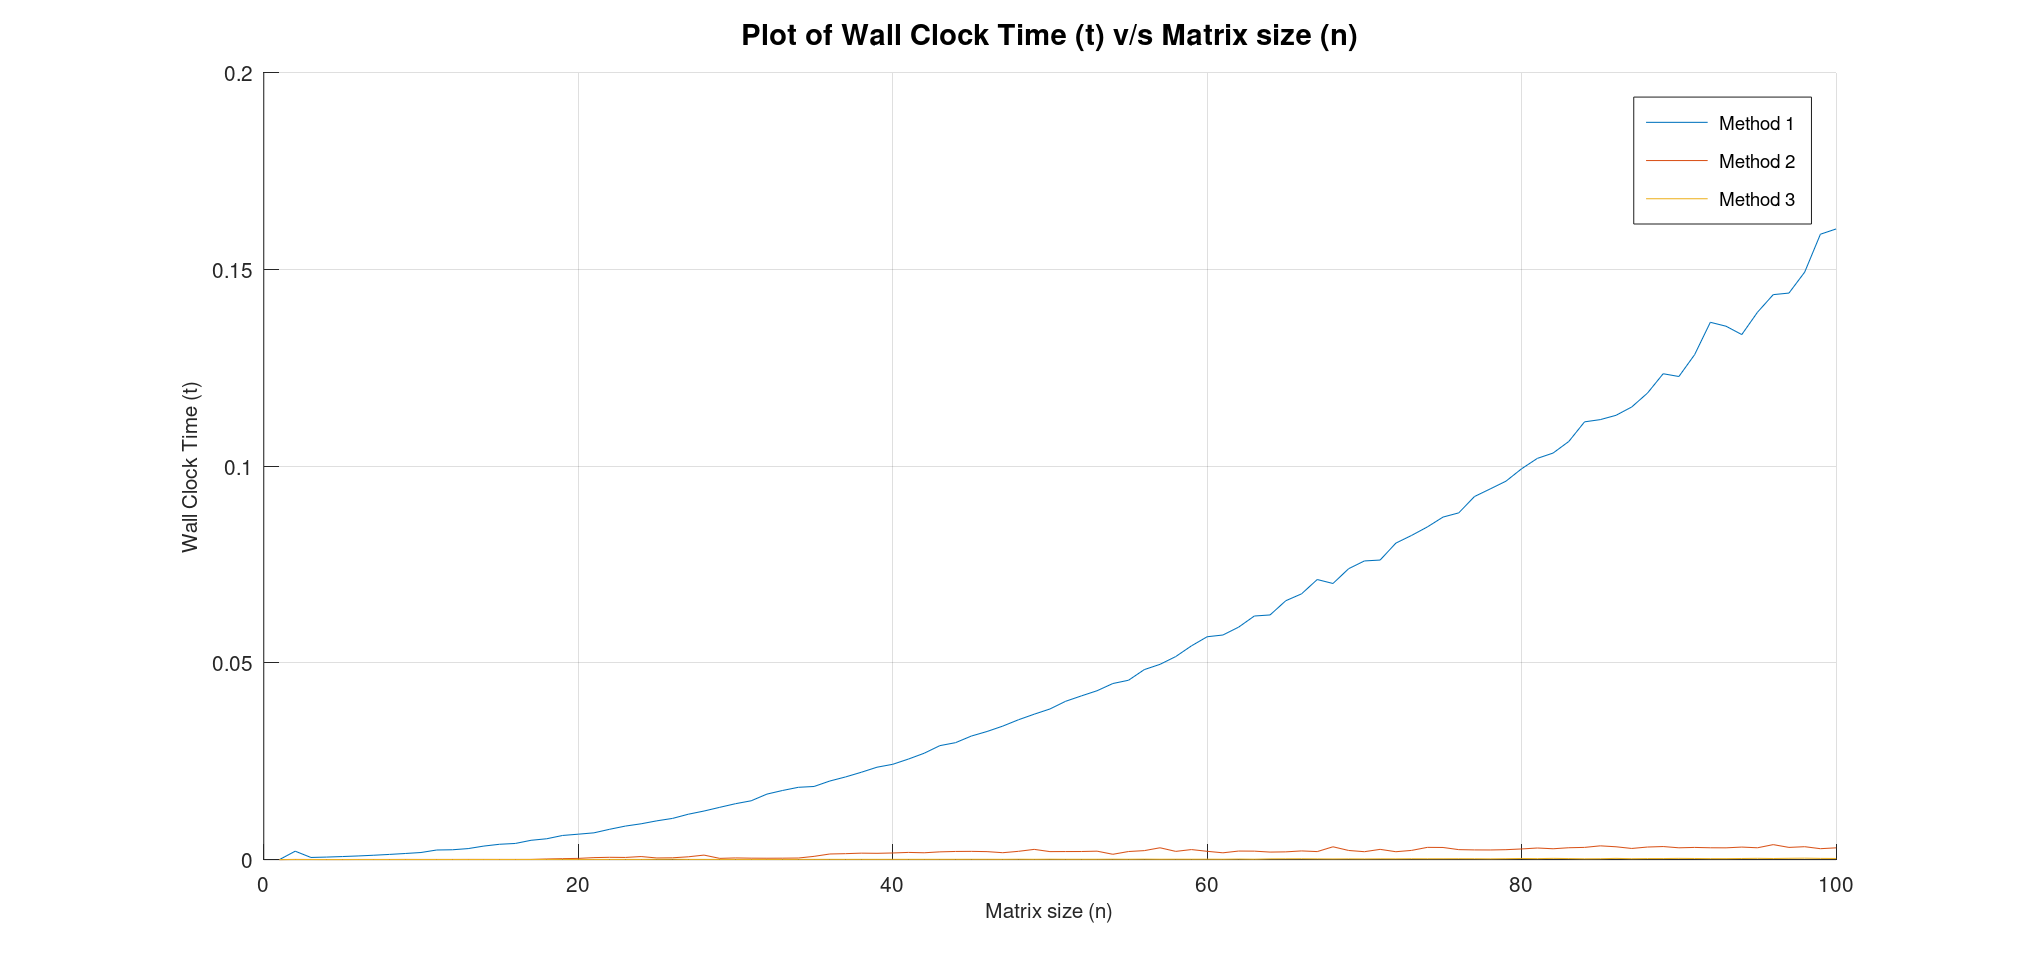
\includegraphics[scale=0.2]{Figure_2.png}
		}
	\end{center}
	\caption{Plot of Wall Clock Time (t) v/s Matrix size (n)}
\end{figure}
\section{Regression Analysis:}
Linear regression analysis is used to predict the value of a variable based on the value of another variable. The variable you want to predict is called the dependent variable. The variable you are using to predict the other variable's value is called the independent variable.
\subsection{A brief overview on Linear Regression:}
Linear Regression is a machine learning algorithm based on supervised learning. It performs a regression task. Regression models a target prediction value based on independent variables. It is mostly used for finding out the relationship between variables and forecasting. Different regression models differ based on – the kind of relationship between dependent and independent variables they are considering, and the number of independent variables getting used.\\
\\Linear regression performs the task to predict a dependent variable value (y) based on a given independent variable (x). So, this regression technique finds out a linear relationship between x (input) and y (output). Hence, the name is Linear Regression.\\
\\Linear regression can be further divided into two types of the algorithm:
\begin{itemize}
\item \textbf{Simple Linear Regression:} If a single independent variable is used to predict the value of a numerical dependent variable, then such a Linear Regression algorithm is called Simple Linear Regression.
\item \textbf{Multiple Linear regression:} If more than one independent variable is used to predict the value of a numerical dependent variable, then such a Linear Regression algorithm is called Multiple Linear Regression.
\end{itemize}
\\When working with linear regression, our main goal is to find the best fit line that means the error between predicted values and actual values should be minimized. The best fit line will have the least error.
\subsection{Performing Regression Analysis on the Data-Sets given:}
Here we have performed Regression Analysis on the data sets given in the assignment template and we get the following plots for the best fit line for each data set provided to us. We have used Regression to predict the value of a variable based on the value of another variable. The variable you want to predict is called the dependent variable. The variable you are using to predict the other variable's value is called the independent variable.
\begin{figure}[!ht]
	\begin{center}
		\framebox{
			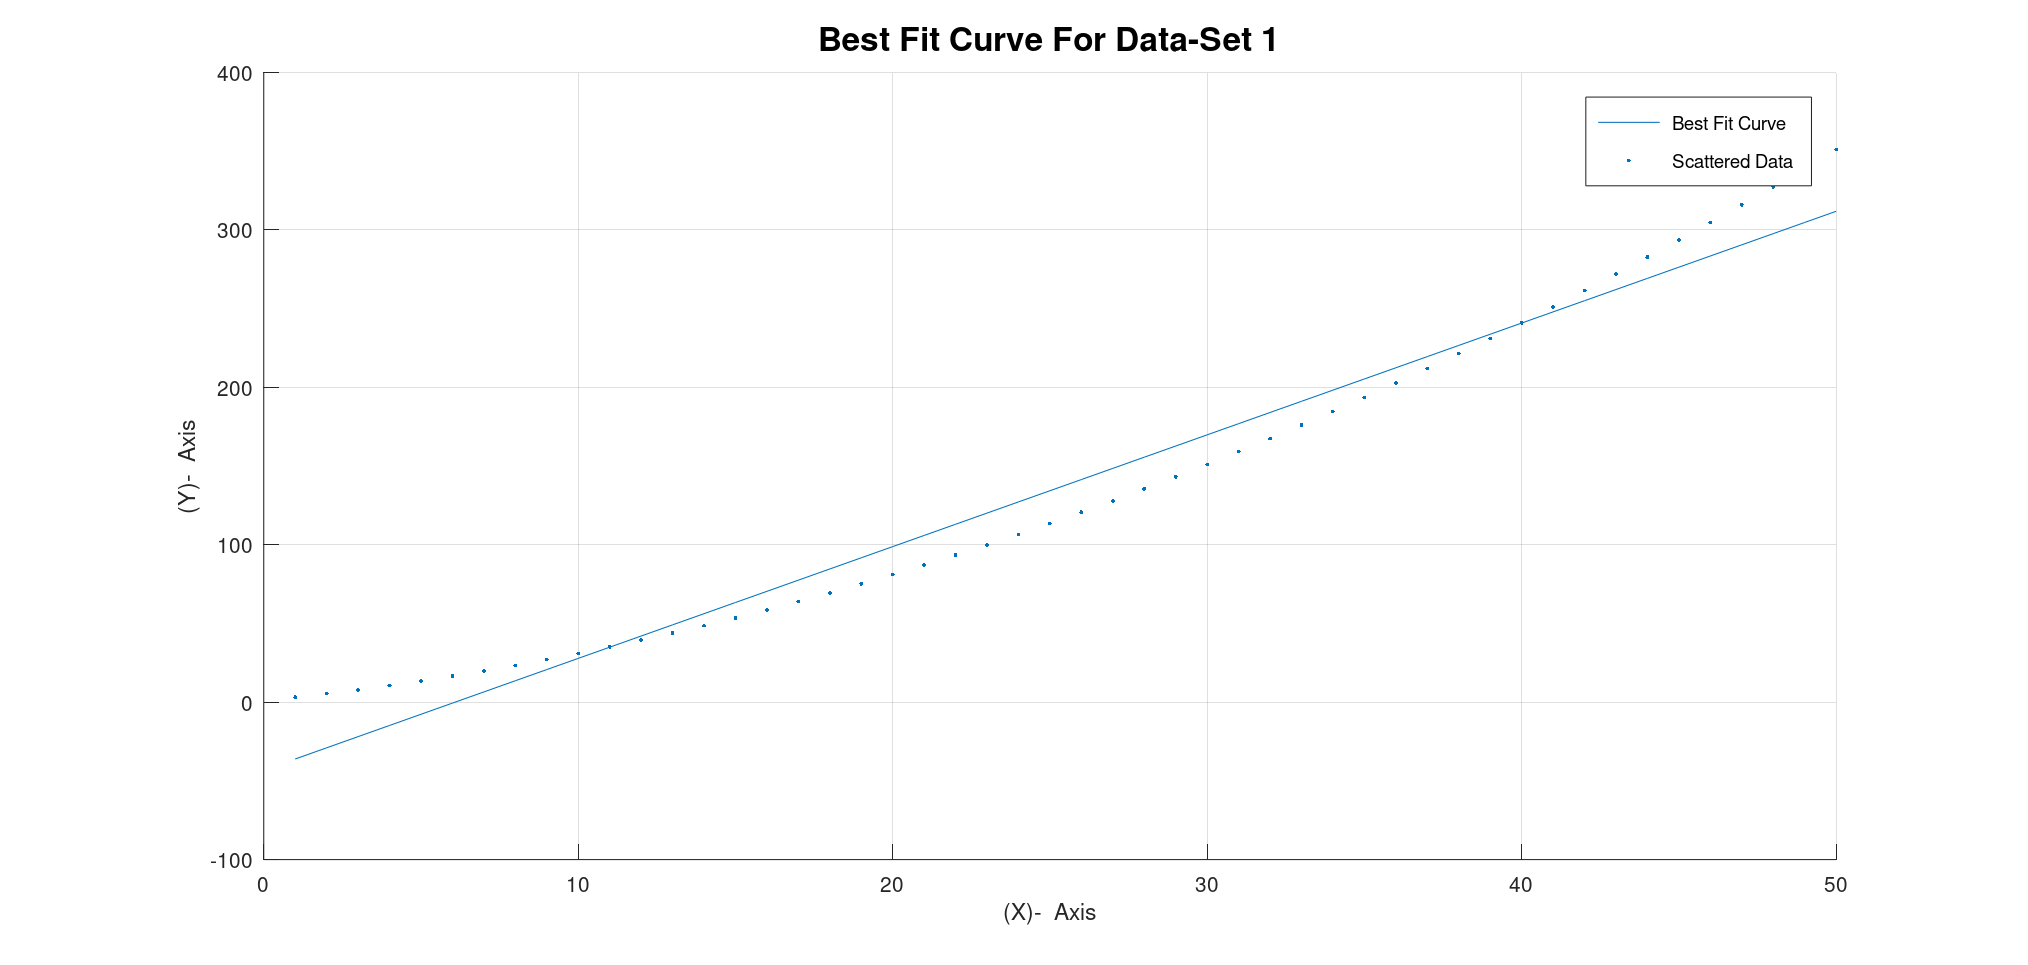
\includegraphics[scale=0.2]{Figure_3.png}
		}
	\end{center}
	\caption{Regression plot for Data-Set 1}
\end{figure}
\begin{figure}[!ht]
	\begin{center}
		\framebox{
			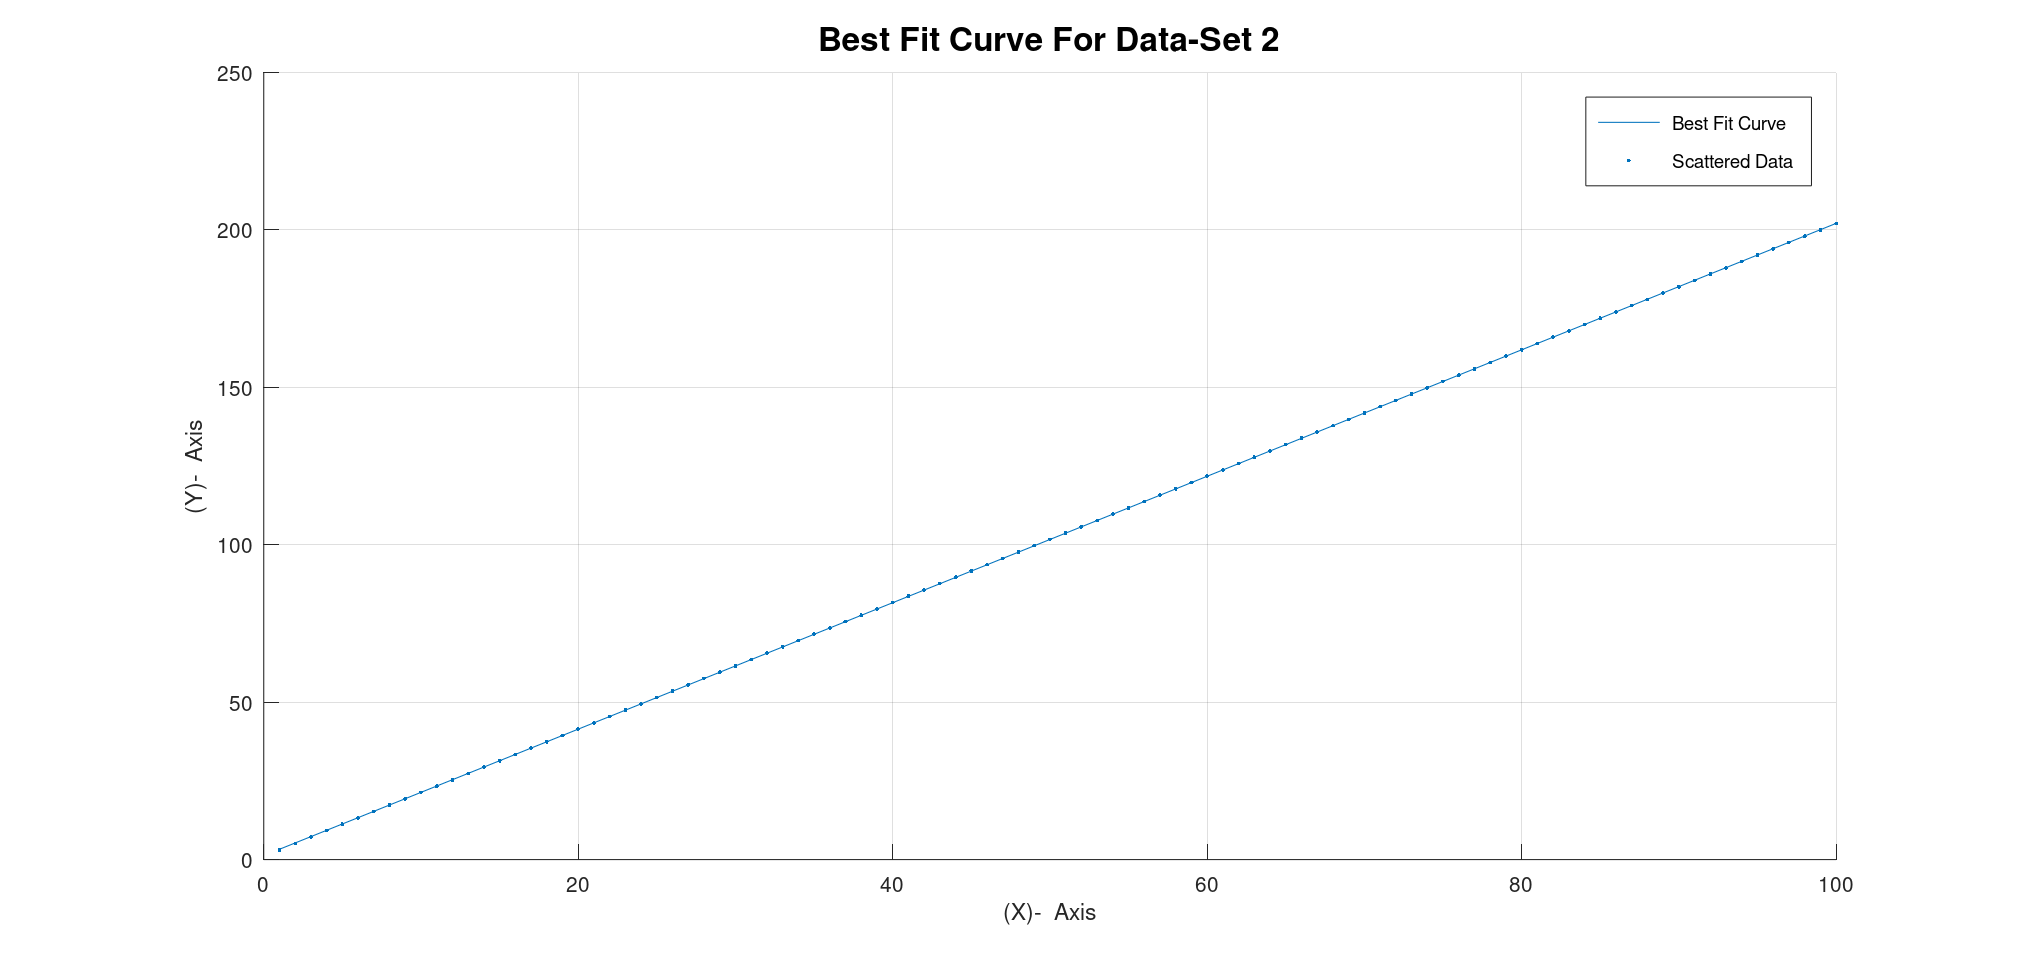
\includegraphics[scale=0.2]{Figure_4.png}
		}
	\end{center}
	\caption{Regression plot for Data-Set 2}
\end{figure}
\clearpage
\begin{figure}[!ht]
	\begin{center}
		\framebox{
			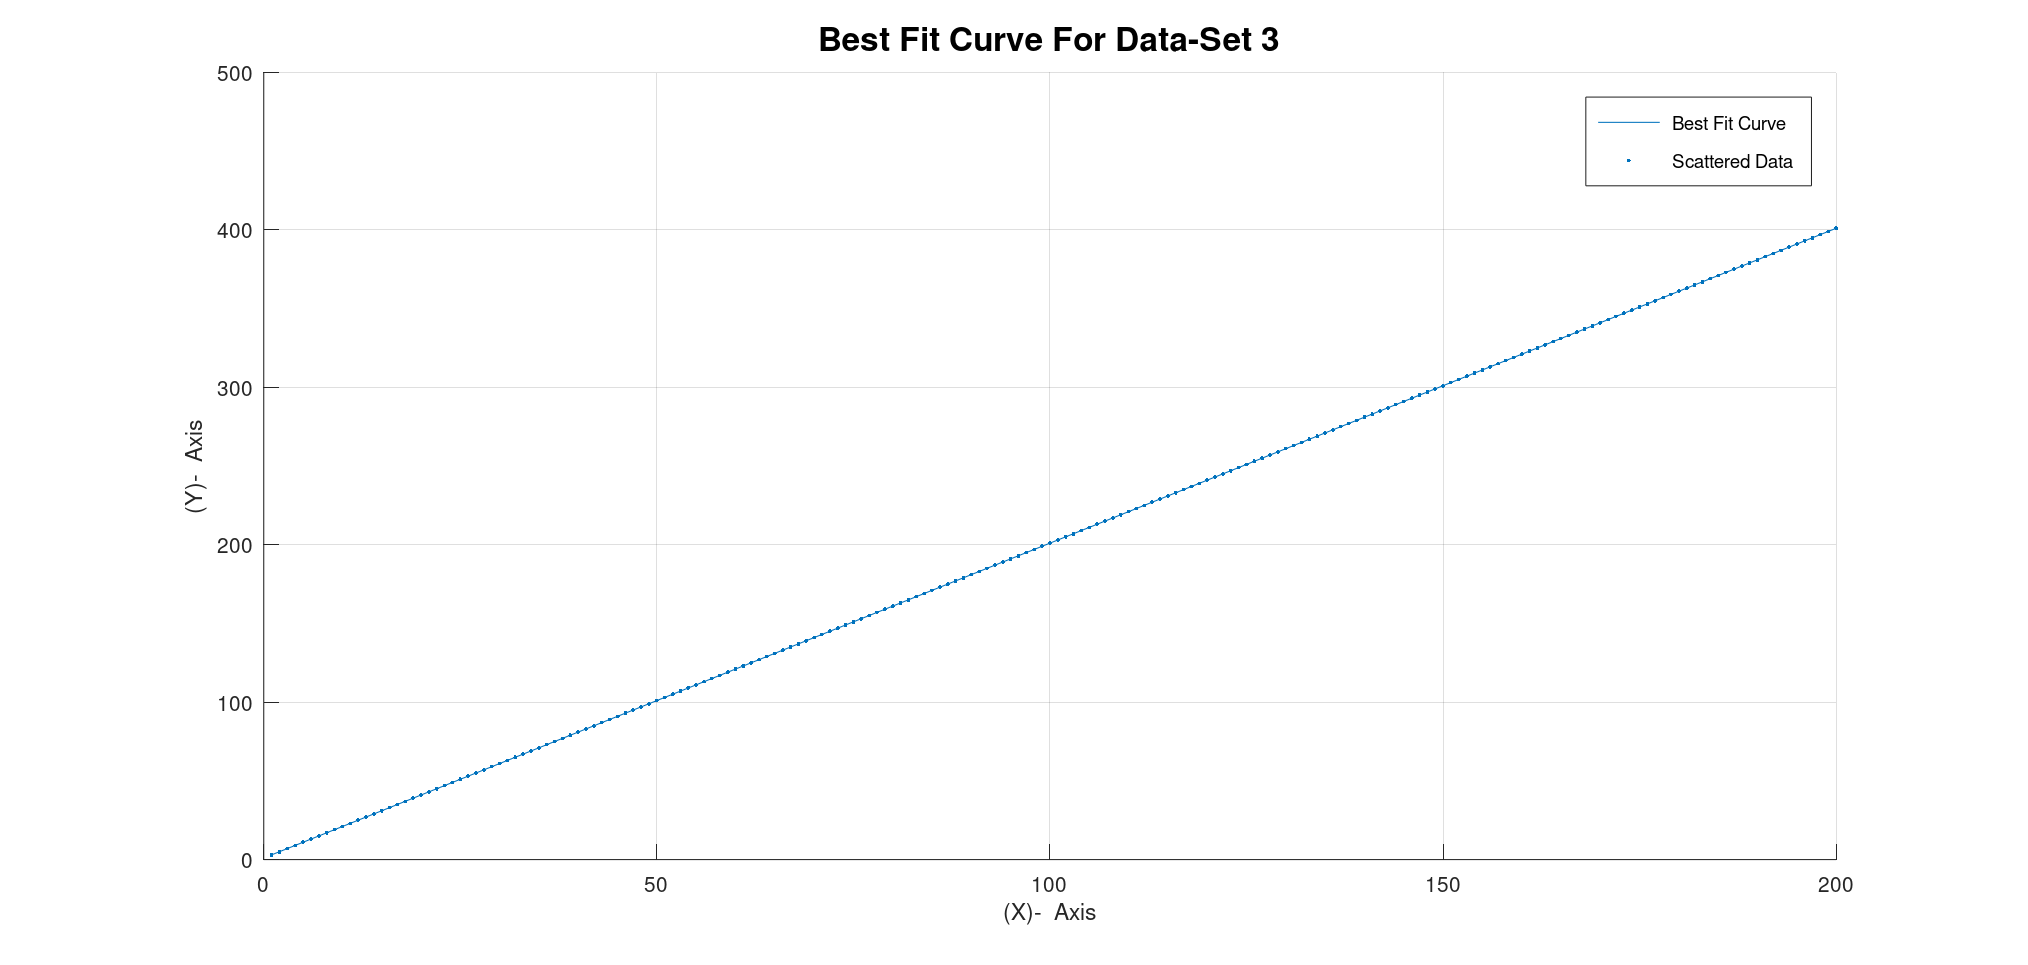
\includegraphics[scale=0.2]{Figure_5.png}
		}
	\end{center}
	\caption{Regression plot for Data-Set 3}
\end{figure}
\subsection{Tables for the Data-Sets:}
In this section we have represented the output tables for the data sets where the rows are 50, 100, 200 and the columns indicate the values of m and c, and based on the values, we infer that the nature of the data provided for the $1^{st}$ data set; when the rows increase there is a drastic change in the values of 'm' and 'c' compared to the other two data sets which represent a more linear variation. We confirm the statement from the result of the Regression Analysis performed on the given data sets represented in the previous subsection. 
\begin{table}[!ht]
	\begin{center}
\begin{tabular}{|c|r|l|}
\hline
Rows & m & c \\
\hline
50 & 7.1000 & -43.2000 \\
100 & 12.1000 & -170.7000 \\
200 & 22.1000 & -675.7000 \\
\hline
\end{tabular}
	\caption{Output Table for $1^{st}$ data set}
	\label{tab:progs}
	\end{center}
\end{table}
\begin{table}[!ht]
	\begin{center}
\begin{tabular}{|c|r|l|}
\hline
Rows & m & c \\
\hline
50 & 2.0111 & 1.1956 \\
100 & 2.0079 & 1.2719 \\
200 & 2.0056 & 1.3810 \\
\hline
\end{tabular}
	\caption{Output Table for $2^{nd}$ data set}
	\label{tab:progs}
	\end{center}
\end{table}
\clearpage
\begin{table}[!ht]
	\begin{center}
\begin{tabular}{|c|r|l|}
\hline
Rows & m & c \\
\hline
50 & 2.0000 & 1.0049 \\
100 & 2.0000 & 1.0047 \\
200 & 2.0000 & 1.0050 \\
\hline
\end{tabular}
	\caption{Output Table for $3^{rd}$ data set}
	\label{tab:progs}
	\end{center}
\end{table}
\subsection{Best Fit Curve for Data-Set 1:}
The model that would work for the $1^{st}$ data set instead of a linear curve is a best fit curve (non-linear) because the the variation of the regression analysis performed on data set 1 is not linear. Hence the hypothesis for the given model is proved.
\begin{figure}[!ht]
	\begin{center}
		\framebox{
			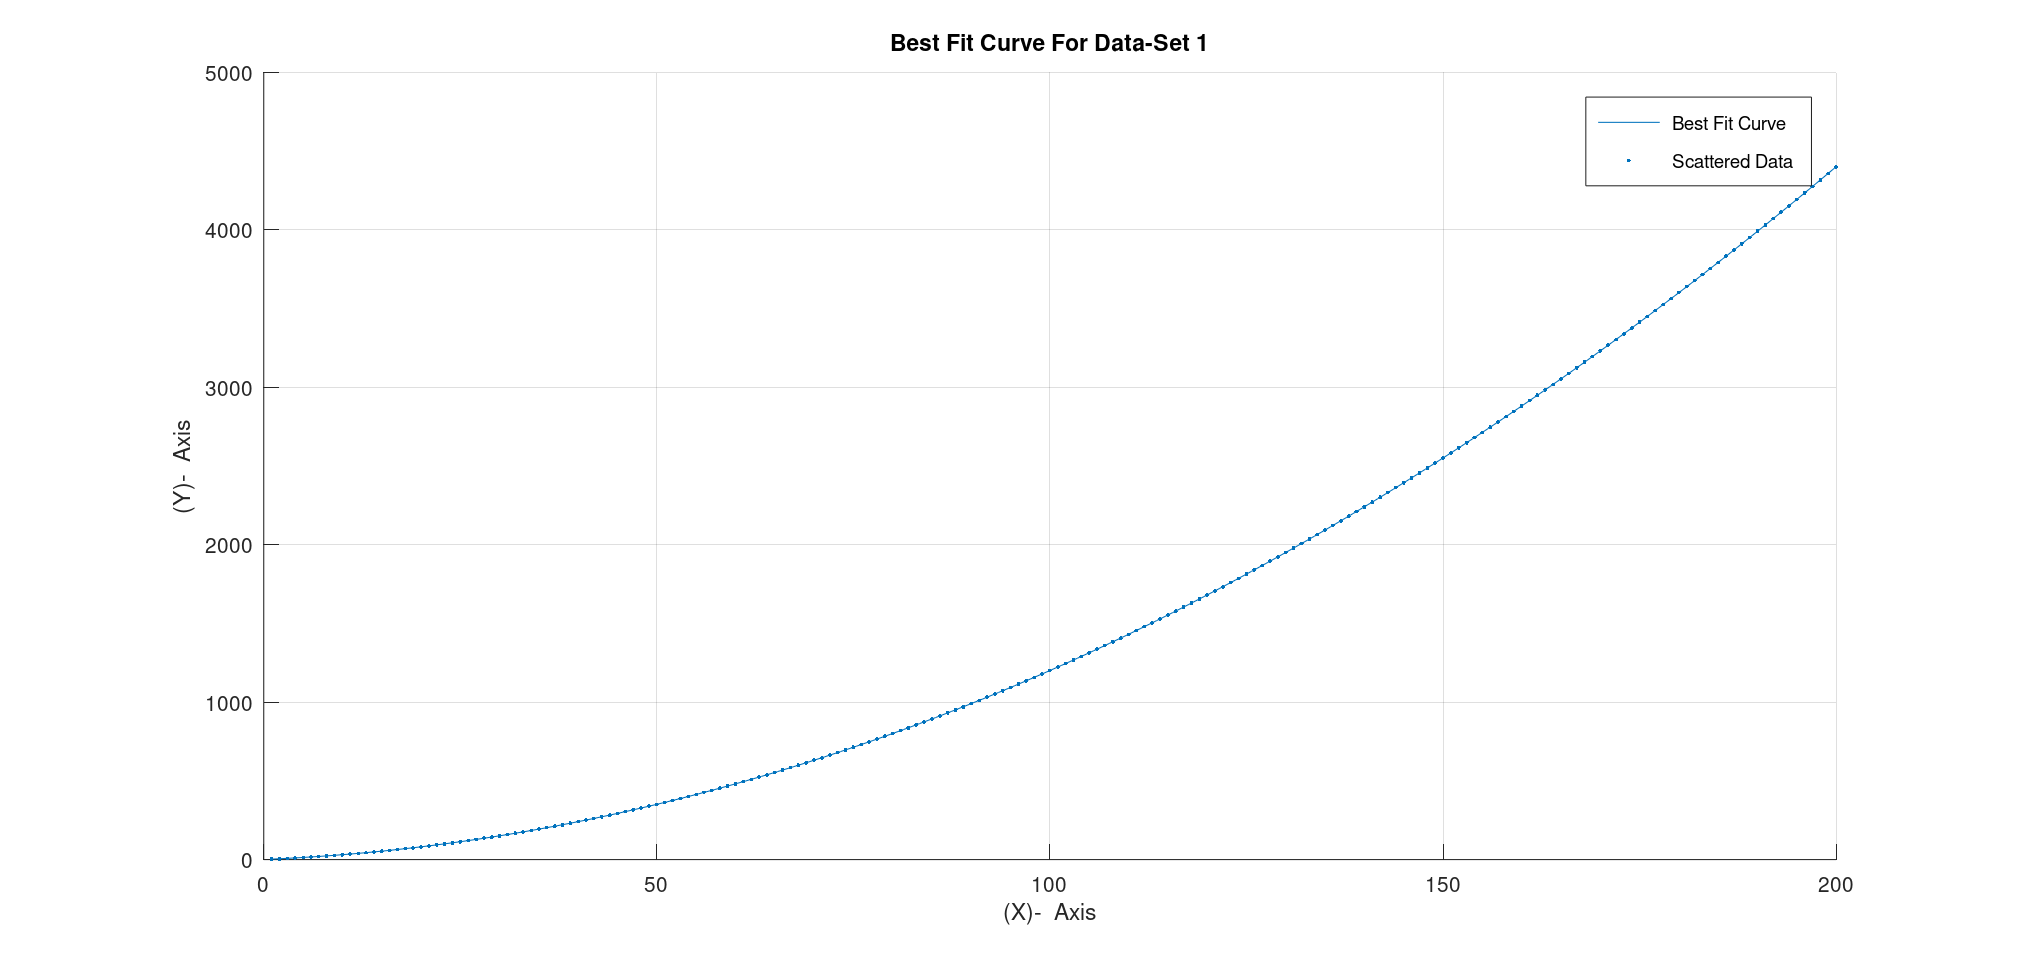
\includegraphics[scale=0.2]{Figure_6.png}
		}
	\end{center}
	\caption{Best Fit Curve for Data-Set 1}
\end{figure}
\end{document}